\newpage
\section{Diskussion}
\label{sec:diskussion}
Beginnend mit den Temperaturprofilen der Wärmetauscher für die Reihen- und Parallelschaltung werden an dieser Stelle die Messergebnisse diskutiert und bewertet. Die in der Abbildung \ref{dia:temp_profil} dargestellten Temperaturverläufe, welche über den Rohrabschnitt aufgetragen wurden,  geben erste Indizien zur Bewertung der beiden Fahrweisen. Es zeigt sich, dass die Temperaturverläufe für den parallelen Betrieb deutlich steiler zulaufen als für die Reihenschaltung. Zu erkennen ist ebenfalls, dass die Temperaturdifferenzen der Parallelschaltung größer sind, als die der Reihenschaltung. Somit lässt sich die Vermutung aufstellen, dass die Parallelschaltung die effizientere Wärmeübertragung für die jeweils eingestellten Volumina liefert. Jedoch sollte beachtet werden, dass für beide Verfahren unterschiedliche Volumenströme gefahren werden. Somit kann anhand dieses Diagramms lediglich die Fahrweise mit den entsprechenden Betriebsparametern verglichen werden. Es gibt jedoch keine Auskunft über den Vergleich von Reihen- und Parallelschaltung.\\

Anhand der Wärmeströme lassen sich nun beide Fahrweisen quantitativ unterscheiden. Die Korrektur der Volumenströme ist hierbei notwendig und gibt Auskunft über den Fehler der Messungen am jeweiligen System. An dieser Stelle zeigt sich, dass über die Parallelschaltung, in Bezug auf die Menge an übertragener Wärme,  effizienter erscheint als die Reihenschaltung. Doch dass lediglich mehr Wärme übertragen wird, gibt noch keine Aussage über die Effizienz des Schaltung. Es lässt sich jedoch sagen, dass offensichtlich in der Parallelschaltung mehr Wärme übertragen und somit abgeführt werden kann, als es für die Reihenschaltung der Fall ist.\\

Zieht man in die Betrachtung nun auch die Wirtschaftlichkeit der jeweiligen Fahrweise mit ein, so setzt man die übertragene Wärmemenge in ein Verhältnis zur benötigen elektrischen Leistung für die Förderung des Fluides. Wirtschaftlichkeit bedeutet in diesem Fall, dass maximal viel Wärme übertragen wird, für einen minimalen Einsatz an elektrischer Leistung für die Kreiselpumpe. Demnach ist das Ziel möglichst hohe Werte für dieses Verhältnis zu erreichen. Es zeigt sich, dass die Werte für die Parallelschaltung deutlich wirtschaftlicher erscheinen als die Reihenschaltung, aufgrund der höheren Menge an übertragenen Wärme über den auszugleichenden Druckverlust. Im Gesamtaufbau überzeugt die Parallelschaltung mit einem Ergebnis, welches um 30\% besser ist, als das der Reihenschaltung.
So besticht die Parallelschaltung unter diesem Aspekt, sowohl für die einzelnen Wärmeübertrager, als auch im Gesamtsystem für diesen Versuchsaufbau. \\

Vergleicht man nun zuletzt die Wärmeübergangs- sowie die Wärmedurchgangskoeffizienten zeigt sich die Fahrweise der Reihenschaltung als effektiver. Erkennbar ist dies daran, dass für jeden betrachteten Wärmetauscher der Wert für die übertragene Fläche pro Quadratmeter und Kelvin in der Reihenschaltung höher ist. Auch der Wärmedurchgang, welcher die übertragene Wärme pro Meter Rohrleitung und Kelvin angibt, ist für diesen Versuchsaufbau für die Reihenschaltung größer. Ein Vergleich der Wärmedurchgangskoeffizienten in \mbox{Diagramm \ref{dia:durchng}} verdeutlicht nochmals grafisch, dass die Wärmetauscher im Reihenbetrieb effizienter arbeiten.

\begin{figure}[h!]
	\begin{center}
		\resizebox{0.8\textwidth}{!}{
			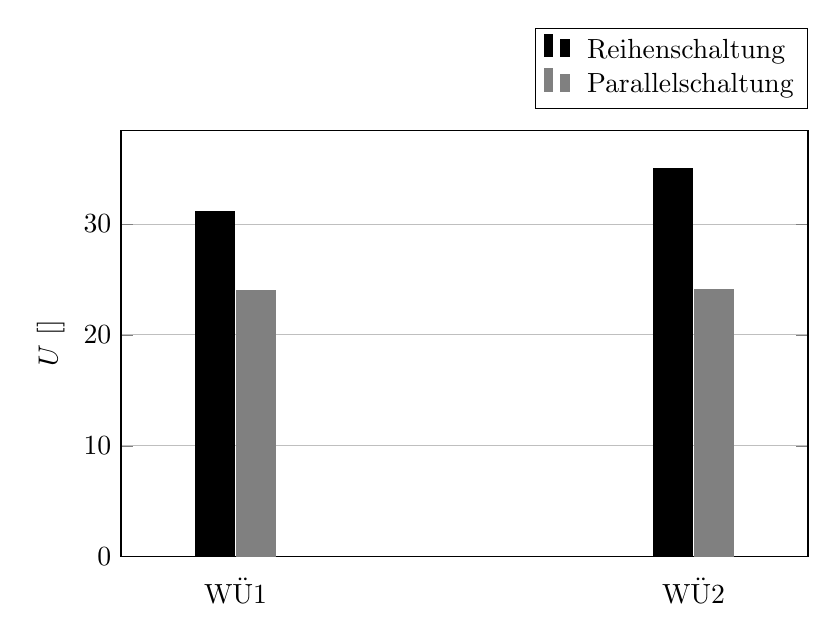
\begin{tikzpicture}
			\begin{axis}[
			width  = 0.85*\textwidth,
			height = 7cm,
			major x tick style = transparent,
			ybar=2*\pgflinewidth,
			bar width=14pt,
			ymajorgrids = true,
			ylabel = {$U \, \left[\si{\watt \per \meter\per\kelvin}\right]$},
			symbolic x coords={WÜ1,WÜ2},
			xtick = data,
			scaled y ticks = false,
			enlarge x limits=0.25,
			ymin=0,
			legend cell align=left,
			legend style={
				at={(1,1.05)},
				anchor=south east,
				column sep=1ex
			}
			]
			%Reihenschaltung
			\addplot[style={black,fill=black,mark=none}]
			coordinates {(WÜ1, 31.13) (WÜ2,34.98)};
			
			%Paralaleschaltung
			\addplot[style={gray,fill=gray,mark=none}]
			coordinates {(WÜ1,23.97) (WÜ2,24.08)};
			
			
			\legend{Reihenschaltung, Parallelschaltung}
			\end{axis}
			\end{tikzpicture}
		}
		\caption{Grafischer Vergleich der Wärmedurchgangskoeffizienten}
		\label{dia:durchng}
	\end{center}
\end{figure}
\FloatBarrier
\newpage
Schlussendlich lässt sich sagen, dass für die gegebenen Betriebsparameter die Parallelschaltung in ihrer Effizienz gegenüber der Reihenschaltung überzeugt. Gerade in Bezug auf die Wirtschaftlichkeit hat die Reihenschaltung keine überzeugenden Argumente für den Betrieb hervorgebracht. Jedoch ist die Reihenschaltung in Bezug auf den Wärmeübergangsprozess effizienter als die Parallelschaltung. Da im Regelfall die benötigte Pumpleistung für den Parallelbetrieb, aufgrund von Strömungswiderständen, größer wäre und sich somit auch der wirtschaftliche Faktor ändern würde, ist es sinnvoller eine Reihenschaltung vorzuziehen. Aus den Ergebnissen des theoretischen Versuches für dieses Protokoll ist jedoch laut dem wirtschaftlichen Aspekt die Parallelschaltung vorzuziehen.

Der berechnete Wärmeverlust entspricht mit den in Gleichung \eqref{gl:Energie-eingesetzt} berechneten \SI{637,5}{\watt} 52\% der Heizleistung. Dies ist aufgrund der vielen un-isolierten Bereiche an der Kolonne plausibel.